\section{Результаты}

В основной спецификации используется совместный линейный фильтр Калмана:
\[
q_{t+1}=Aq_t+\varepsilon_{t+1},
\qquad
o_t=M_\phi q_t+\nu_t.
\]
Матрица наблюдения \(M_\phi\) задаёт информационное состояние, а динамика \(A\) и ковариация
шоков остаются общими. Поэтому неполная наблюдаемость не сводится к независимому сглаживанию
отдельных рядов. Скалярный фильтр используется только как техническая проверка.

\subsection{Качество фильтрации}

Совместный фильтр существенно снижает ошибку измерения. Для агрегатного информационного
состояния RMSE инфляции падает с \(0.000896\) у шумного наблюдения до \(0.000276\), для выпуска
-- с \(0.002679\) до \(0.000900\), для потребления -- с \(0.001150\) до \(0.000367\). При
добавлении распределительных сигналов RMSE средней MPC равен \(0.001793\) против \(0.005713\)
у шумного наблюдения, RMSE доли низколиквидных домохозяйств -- \(0.000962\) против \(0.005465\),
RMSE процентной экспозиции -- \(0.000123\) против \(0.000640\).

\subsection{Основная оценка}

Для каждого информационного состояния заново настраивается линейное правило ставки. В этой версии
используется непрерывная минимизация validation loss внутри класса линейных правил; старый
случайный перебор сохранён как базовая проверка.

\begin{table}[h!]
\centering
\caption{Потери политики по информационным состояниям}
\resizebox{\textwidth}{!}{%
\begin{tabular}{lrrrr}
\toprule
Информационное состояние & Число траекторий & Средние потери & Нижняя граница & Верхняя граница \\
\midrule
Текущие агрегаты & 300 & 0.000533 & 0.000484 & 0.000586 \\
История агрегатов & 300 & 0.000522 & 0.000474 & 0.000575 \\
Фильтрованные агрегаты & 300 & 0.000433 & 0.000399 & 0.000471 \\
Наблюдаемые распределительные показатели & 300 & 0.000359 & 0.000327 & 0.000394 \\
Фильтрованные агрегаты + MPC & 300 & 0.000375 & 0.000347 & 0.000408 \\
Фильтрованные агрегаты + низкая ликвидность & 300 & 0.000372 & 0.000345 & 0.000403 \\
Фильтрованные агрегаты + процентная экспозиция & 300 & 0.000373 & 0.000346 & 0.000403 \\
Фильтрованные распределительные показатели & 300 & 0.000378 & 0.000348 & 0.000411 \\
Полная информация & 300 & 0.000205 & 0.000195 & 0.000215 \\
\bottomrule
\end{tabular}
}
\end{table}

Переход от текущих агрегатов к фильтрованным агрегатам снижает средние потери с \(0.000533\) до
\(0.000433\). Добавление распределительных статистик сверх фильтрованных агрегатов снижает
потери до \(0.000378\). Отдельные статистики дают близкий эффект: MPC, доля низколиквидных
домохозяйств и процентная экспозиция по отдельности дают потери около \(0.00037\).

\subsection{Парные сравнения}

\begin{table}[h!]
\centering
\caption{Парные разности потерь на одинаковых тестовых траекториях}
\resizebox{\textwidth}{!}{%
\begin{tabular}{lrrrr}
\toprule
Сравнение & Снижение потерь & Нижняя граница & Верхняя граница & Доля выигрышей \\
\midrule
Фильтрованные агрегаты против текущих агрегатов & 0.000099 & 0.000060 & 0.000140 & 0.613 \\
Наблюдаемые распределительные показатели против текущих агрегатов & 0.000174 & 0.000132 & 0.000216 & 0.703 \\
Фильтрованные агрегаты + MPC против фильтрованных агрегатов & 0.000058 & 0.000037 & 0.000079 & 0.570 \\
Фильтрованные агрегаты + низкая ликвидность против фильтрованных агрегатов & 0.000061 & 0.000041 & 0.000081 & 0.597 \\
Фильтрованные агрегаты + процентная экспозиция против фильтрованных агрегатов & 0.000061 & 0.000041 & 0.000081 & 0.593 \\
Все фильтрованные распределительные показатели против фильтрованных агрегатов & 0.000055 & 0.000027 & 0.000083 & 0.587 \\
Полная информация против текущих агрегатов & 0.000328 & 0.000282 & 0.000379 & 0.890 \\
\bottomrule
\end{tabular}
}
\end{table}

Главная оценка предельной ценности распределительной информации положительна:
\[
J(s^{filt-agg})-J(s^{filt-dist})=0.000055.
\]
Доверительный интервал для разности \(J(s^{filt-dist})-J(s^{filt-agg})\) лежит ниже нуля:
\([-0.000083,-0.000027]\). Значит, в локальной HANK/SSJ-среде распределительные статистики
снижают потери сверх фильтрованных агрегатов, но эффект остаётся умеренным.

\subsection{Информационная граница}

Чтобы показать не только отдельные попарные сравнения, но и всю лестницу информационных состояний,
строится информационная граница. Уровень 0 соответствует текущим агрегатам, уровень 1 -- истории
агрегатов, уровень 2 -- фильтрованным агрегатам, уровень 3 -- лучшему одному распределительному
сигналу, уровень 4 -- всем фильтрованным распределительным сигналам, уровень 5 -- полной
информации.

В основной спецификации потери убывают с \(0.000533\) для текущих агрегатов до \(0.000433\) для
фильтрованных агрегатов и до \(0.000372\) для лучшего одиночного распределительного сигнала. Все
распределительные сигналы вместе дают \(0.000378\), то есть в данной калибровке не доминируют
лучший одиночный сигнал. Это важная оговорка: работа не утверждает, что механическое добавление
всех распределительных показателей всегда лучше. Предельная ценность распределительной информации
появляется тогда, когда конкретный сигнал помогает оценить будущую трансмиссию ставки.

\begin{figure}[h!]
\centering
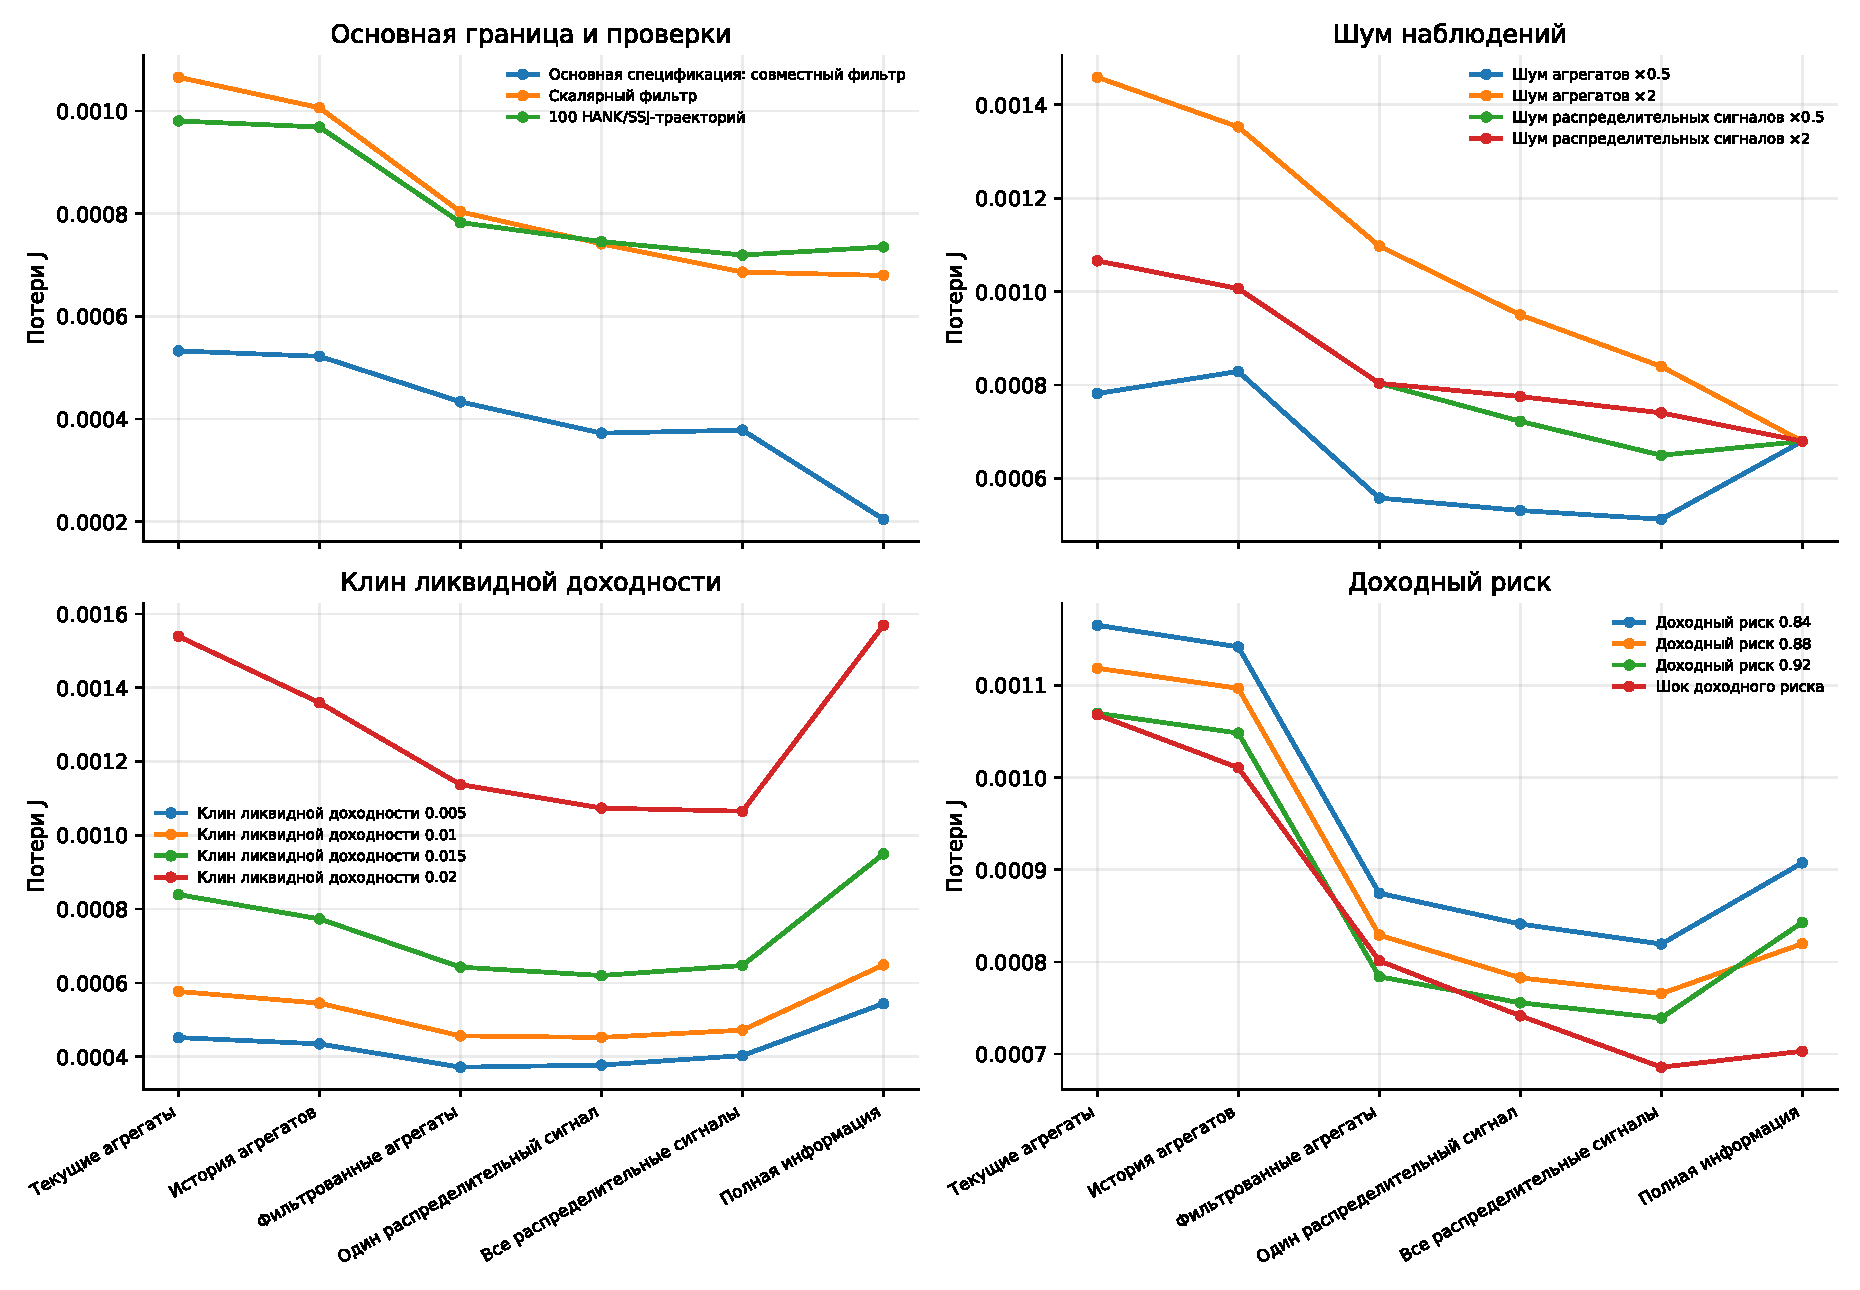
\includegraphics[width=\textwidth]{figures/fig_information_frontier.pdf}
\caption{Информационная граница: потери по уровням доступной информации}
\end{figure}

\begin{figure}[h!]
\centering
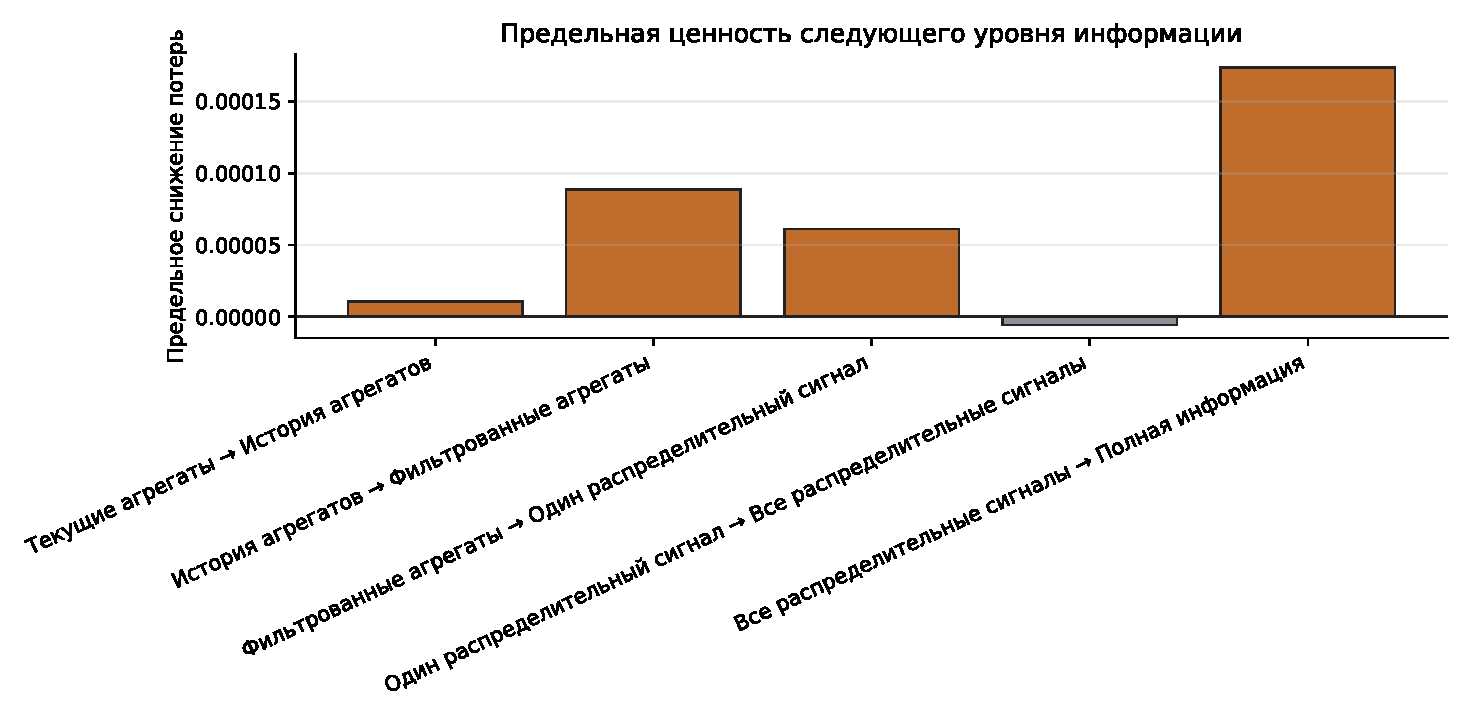
\includegraphics[width=\textwidth]{figures/fig_information_marginal_values.pdf}
\caption{Предельная ценность следующего уровня информации}
\end{figure}

\begin{table}[h!]
\centering
\caption{Устойчивость ранжирования информационных уровней}
\resizebox{\textwidth}{!}{%
\begin{tabular}{lrrrr}
\toprule
Проверка & Число вариантов & Средняя ранговая корреляция & Минимальная корреляция & Совпадение лучшего уровня \\
\midrule
Тестовые seed & 6 & 0.950 & 0.800 & 0.667 \\
Совместный фильтр против скалярного & 1 & 0.900 & 0.900 & 0.000 \\
Число траекторий & 1 & 1.000 & 1.000 & 1.000 \\
Шум наблюдений & 4 & 0.975 & 0.900 & 1.000 \\
Клин ликвидной доходности & 4 & 0.750 & 0.600 & 0.250 \\
Доходный риск & 4 & 1.000 & 1.000 & 1.000 \\
Сила распределительного сигнала & 4 & 1.000 & 1.000 & 1.000 \\
\bottomrule
\end{tabular}
}
\end{table}

Ранговая проверка проводится по реализуемым информационным состояниям 0--4; полная информация
остаётся ориентиром, но не включается в ранги старых sensitivity-прогонов. Ранжирование в целом
устойчиво к числу траекторий, шуму наблюдений, доходному риску и силе распределительного сигнала.
Наиболее чувствительная часть -- калибровка клина ликвидной доходности: при слабом клине
распределительная информация может не улучшать правило, а при более сильном канале её ценность
становится положительной.

\subsection{Оптимизация правил}

Смена способа настройки правил существенно влияет на уровни потерь. Например, для фильтрованных
агрегатов старый поиск по сетке даёт test loss \(0.000776\), а непрерывная оптимизация --
\(0.000433\). Для фильтрованного распределительного состояния соответствующие значения равны
\(0.000842\) и \(0.000378\). Поэтому в основной таблице используются результаты непрерывной
оптимизации, а таблица устойчивости сохраняет также старые режимы подбора.

Отдельная проверка показывает, что выигрыш распределительного состояния не является простой
проекцией коэффициентов. Если взять правило, настроенное на распределительном наборе, занулить
распределительные коэффициенты и применить его к фильтрованным агрегатам, средние потери равны
\(0.001858\), тогда как заново настроенное агрегатное правило даёт \(0.000433\). Это подтверждает,
что разные информационные состояния нужно сравнивать после отдельной настройки правила.

\subsection{Устойчивость к классу правила}

Основной результат не должен зависеть от одного специфического класса правил. Поэтому дополнительно
сравниваются несколько разумных альтернатив: правило типа Тейлора, правило Тейлора с потреблением,
правило Тейлора с распределительными показателями, правило с ограничениями на знаки, регуляризованные
линейные правила и малое нелинейное правило. Во всех случаях правила настраиваются на тех же
валидационных траекториях и оцениваются на тех же тестовых траекториях.

\begin{table}[h!]
\centering
\caption{Устойчивость ценности распределительной информации к классу правила}
\resizebox{\textwidth}{!}{%
\begin{tabular}{lrrrr}
\toprule
Класс правила & Снижение потерь & Нижняя граница для \(\Delta J\) & Верхняя граница для \(\Delta J\) & Доля выигрышей \\
\midrule
Правило Тейлора & 0.000058 & -0.000090 & -0.000025 & 0.560 \\
Тейлор + потребление & 0.000079 & -0.000103 & -0.000055 & 0.593 \\
Тейлор + распределительные показатели & 0.000141 & -0.000181 & -0.000103 & 0.610 \\
Правило с ограничениями на знаки & 0.000141 & -0.000181 & -0.000103 & 0.610 \\
Оптимизированное линейное правило & 0.000073 & -0.000101 & -0.000045 & 0.563 \\
Ridge-регуляризация & 0.000073 & -0.000101 & -0.000045 & 0.563 \\
LASSO/ElasticNet & 0.000073 & -0.000101 & -0.000045 & 0.563 \\
\bottomrule
\end{tabular}
}
\end{table}

Во всех основных классах правил предельная ценность распределительной информации остаётся
положительной. Это важно для интерпретации: результат не держится на одной форме линейного правила
и не исчезает при ограничениях на знаки или регуляризации коэффициентов. Малое нелинейное правило
используется только как дополнительная проверка; в текущей реализации оно даёт худший результат и
поэтому не является частью основного аргумента. Тем самым вывод работы остаётся не про преимущество
сложных алгоритмов, а про ценность информационного состояния.

\begin{figure}[h!]
\centering
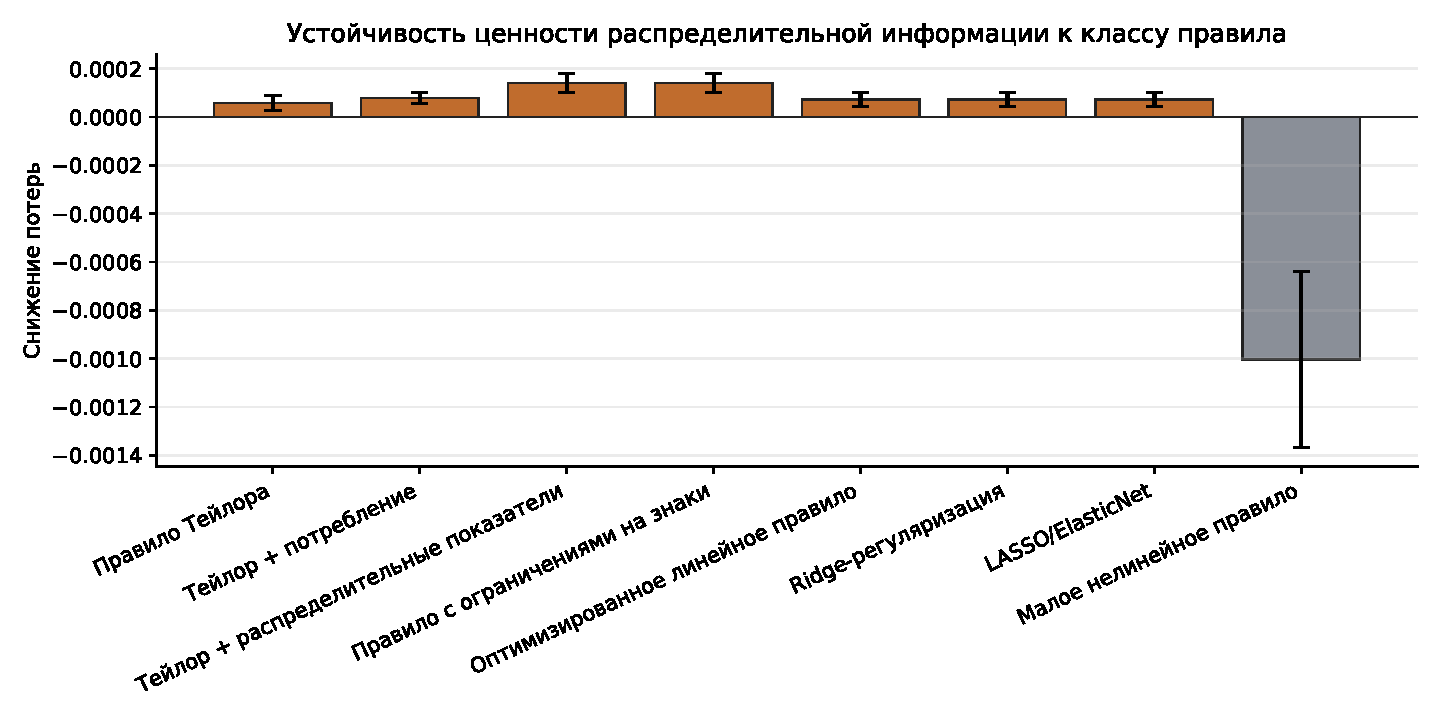
\includegraphics[width=\textwidth]{figures/fig_policy_class_robustness.pdf}
\caption{Снижение потерь при добавлении распределительной информации в разных классах правил}
\end{figure}

\subsection{Идентификационные проверки}

Чтобы отделить ценность информации от механического увеличения числа признаков, проводится
батарея проверок. Во всех вариантах агрегатный блок \(E\pi,EY,EC\) в распределительном
информационном состоянии принудительно приравнен к фильтрованным агрегатам. Меняются только
распределительные признаки.

\begin{table}[h!]
\centering
\caption{Идентификационные проверки распределительных признаков}
\resizebox{\textwidth}{!}{%
\begin{tabular}{lrrrr}
\toprule
Проверка & Снижение потерь & Нижняя граница для \(\Delta J\) & Верхняя граница для \(\Delta J\) & Доля выигрышей \\
\midrule
Фактическая распределительная информация & 0.000038 & -0.000070 & -0.000004 & 0.550 \\
Искусственные признаки с похожей статистикой & -0.000018 & 0.000008 & 0.000029 & 0.440 \\
Перемешивание между сценариями & 0.000003 & -0.000006 & -0.000000 & 0.540 \\
Перемешивание времени внутри сценария & 0.000002 & -0.000008 & 0.000005 & 0.590 \\
Запаздывающие распределительные признаки & -0.000027 & 0.000014 & 0.000040 & 0.393 \\
Будущие сдвинутые распределительные признаки & -0.000030 & 0.000018 & 0.000044 & 0.407 \\
Остаточная распределительная информация & 0.000055 & -0.000084 & -0.000025 & 0.563 \\
\bottomrule
\end{tabular}
}
\end{table}

Ключевой результат здесь -- строка с остаточной распределительной информацией. В ней
распределительные признаки предварительно очищаются от линейной зависимости от фильтрованных
агрегатов на валидационной выборке. Даже после этого снижение потерь остаётся положительным:
\(0.000055\), а интервал для \(\Delta J\) лежит ниже нуля. Напротив, искусственные признаки с
похожей дисперсией, авторегрессией и корреляцией с агрегатами ухудшают правило. Лаговые и
будущие сдвинутые признаки также ухудшают результат. Это говорит против объяснения «правило
выиграло просто потому, что получило больше входов».

\subsection{Сравнительная статика робастности}

Робастность удобно читать не как набор отдельных таблиц, а как ответы на три экономических
вопроса.

Первый вопрос: когда распределительная информация полезна? В старой sensitivity-спецификации при
росте шума агрегатных наблюдений предельная ценность распределительной информации возрастает:
при половинном шуме агрегатов \(MVOI_{dist}=0.000045\), а при удвоенном шуме агрегатов --
\(0.000258\). Напротив, когда шум самих распределительных сигналов растёт, ценность падает:
при половинном шуме распределительных сигналов \(MVOI_{dist}=0.000154\), при удвоенном --
\(0.000063\). Это соответствует основной гипотезе: распределительная информация ценна тогда,
когда она помогает компенсировать неполноту агрегатных сигналов, но сама должна быть достаточно
информативной.

Второй вопрос: когда распределительная информация не полезна? Если распределительная динамика
выключена, \(MVOI_{dist}\) исчезает. При слабом клине ликвидной доходности результат также
отрицателен или близок к нулю: при \(\omega=0.005\) \(MVOI_{dist}=-0.000031\), при
\(\omega=0.010\) -- \(-0.000016\), при \(\omega=0.015\) -- \(-0.000004\). При более сильном
канале, \(\omega=0.020\), показатель становится положительным и равен \(0.000072\). Поэтому
отрицательные случаи не являются провалом результата: они показывают, что распределительная
информация ценна не всегда, а именно когда распределительный канал достаточно силён.

Третий вопрос: через какой компонент функции потерь проходит выигрыш? В основной joint-filter
спецификации почти весь выигрыш от распределительной информации сверх фильтрованных агрегатов
идёт через разрыв выпуска. Из общего снижения \(0.000055\) около \(0.000048\) приходится на
компонент выпуска, тогда как инфляция даёт \(0.000004\), потребление -- \(0.000004\), а
сглаживание ставки почти не меняется. Экономически это означает, что распределительные сигналы
помогают не за счёт более агрессивной ставки, а за счёт лучшего выбора реакции на будущую
реальную трансмиссию.

\begin{figure}[h!]
\centering
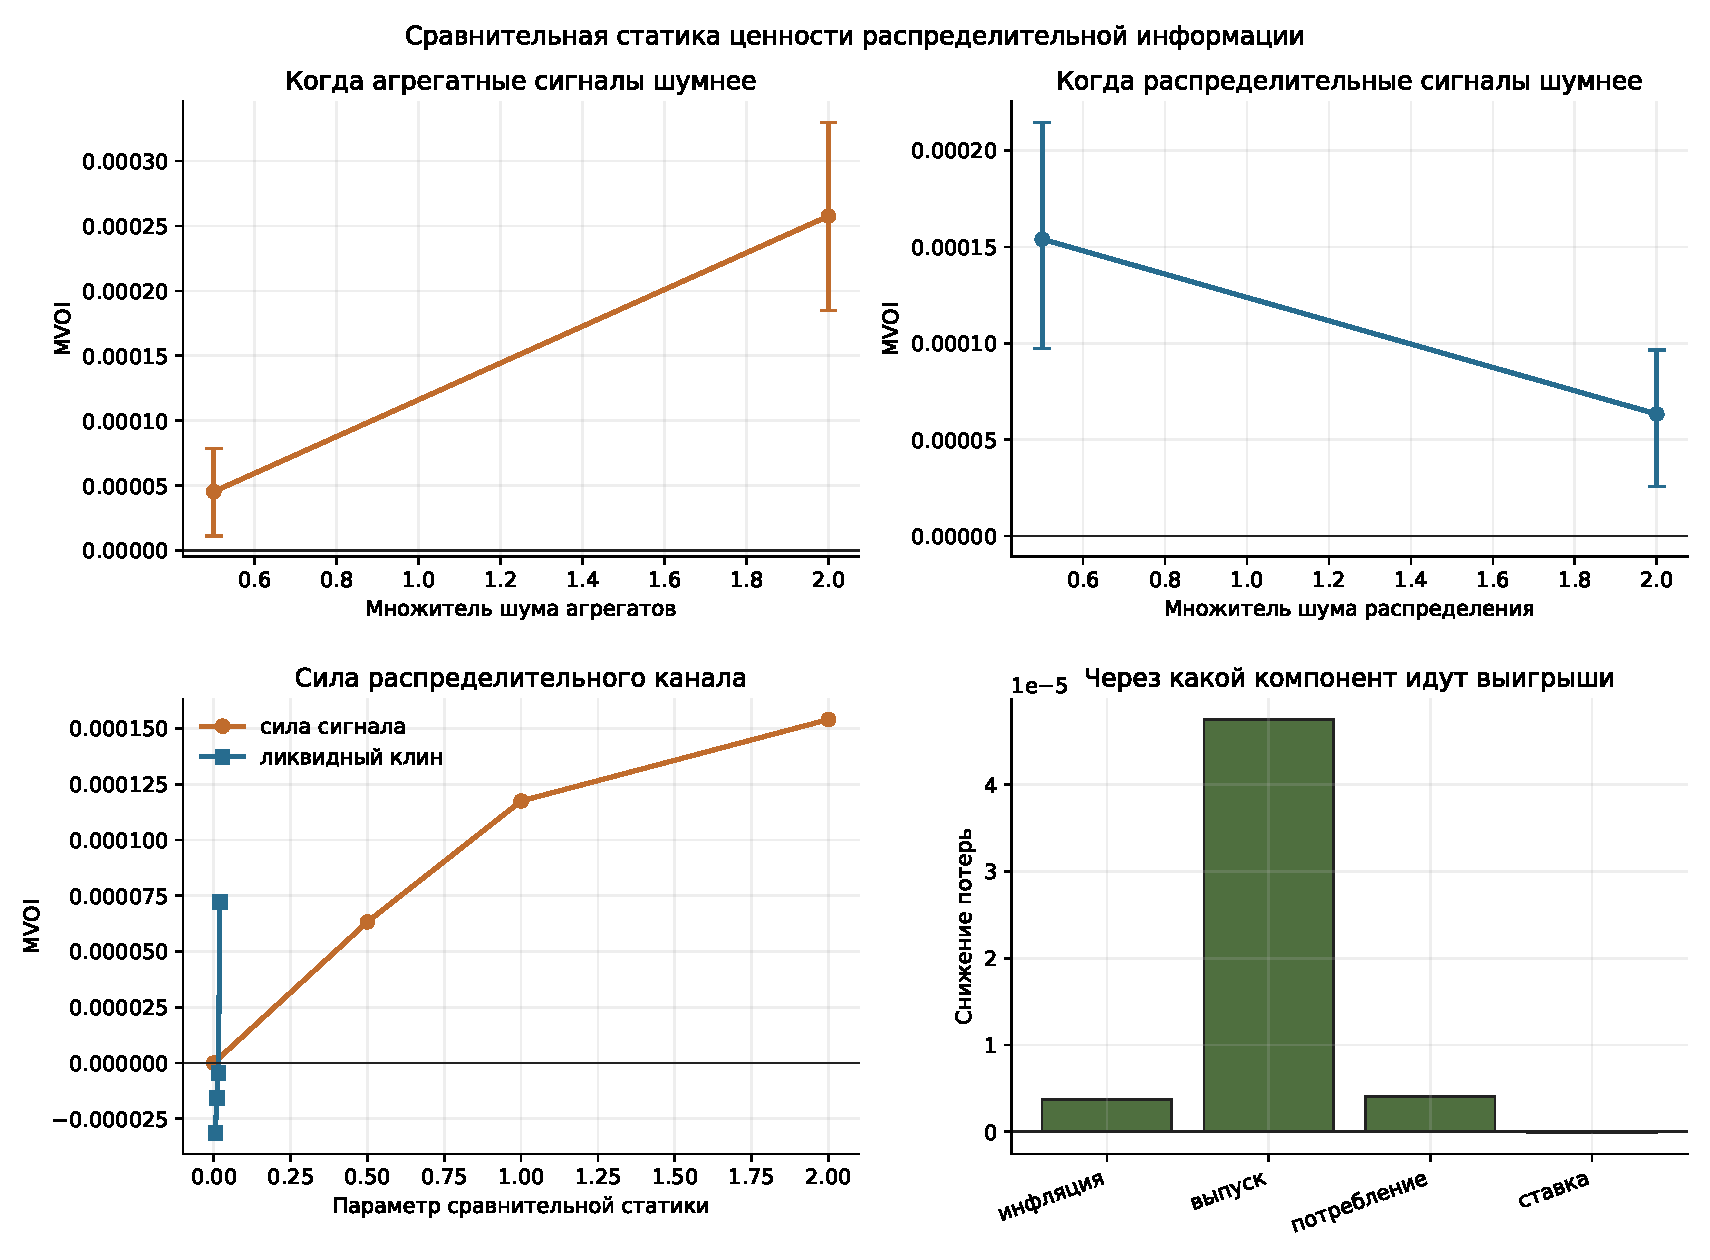
\includegraphics[width=\textwidth]{figures/fig_robustness_comparative_statics.pdf}
\caption{Сравнительная статика ценности распределительной информации}
\end{figure}

Часть сравнительной статики была посчитана в старой скалярной фильтровой спецификации. Поэтому
эти проверки используются как направленная экономическая робастность, а не как замена основной
оценки. Основная оценка статьи остаётся спецификацией с совместным фильтром Калмана и
непрерывной настройкой линейных правил.

\subsection{Механизм через локально оптимальную ставку}

Для проверки механизма строится локально SSJ-оптимальная траектория ставки \(i_t^{*,SSJ}\).
Затем оценивается, какие информационные состояния лучше предсказывают эту ставку на независимых
траекториях.

\begin{table}[h!]
\centering
\caption{Прогноз локально SSJ-оптимальной ставки}
\resizebox{\textwidth}{!}{%
\begin{tabular}{lrrrrr}
\toprule
Спецификация & RMSE & OOS \(R^2\) & \(\Delta\)RMSE vs aggregates & p-value & Directional accuracy \\
\midrule
Фильтрованные агрегаты & 0.000945 & 0.067 &  &  & 0.582 \\
Фильтрованные агрегаты + MPC & 0.000937 & 0.084 & -0.000008 & 0.00025 & 0.596 \\
Фильтрованные агрегаты + низкая ликвидность & 0.000936 & 0.085 & -0.000009 & 0.00025 & 0.599 \\
Фильтрованные агрегаты + процентная экспозиция & 0.000937 & 0.084 & -0.000009 & 0.00025 & 0.597 \\
Фильтрованные распределительные показатели & 0.000924 & 0.109 & -0.000022 & 0.00025 & 0.610 \\
\bottomrule
\end{tabular}
}
\end{table}

Распределительные признаки улучшают прогноз локально оптимальной ставки сверх фильтрованных
агрегатов. Полное распределительное состояние снижает RMSE с \(0.000945\) до \(0.000924\) и
повышает вневыборочный \(R^2\) с \(0.067\) до \(0.109\). После удаления части оптимальной ставки,
объясняемой агрегатами, остаточные распределительные признаки всё ещё объясняют около \(2.9\%\)
остаточной вариации.

\begin{figure}[h!]
\centering
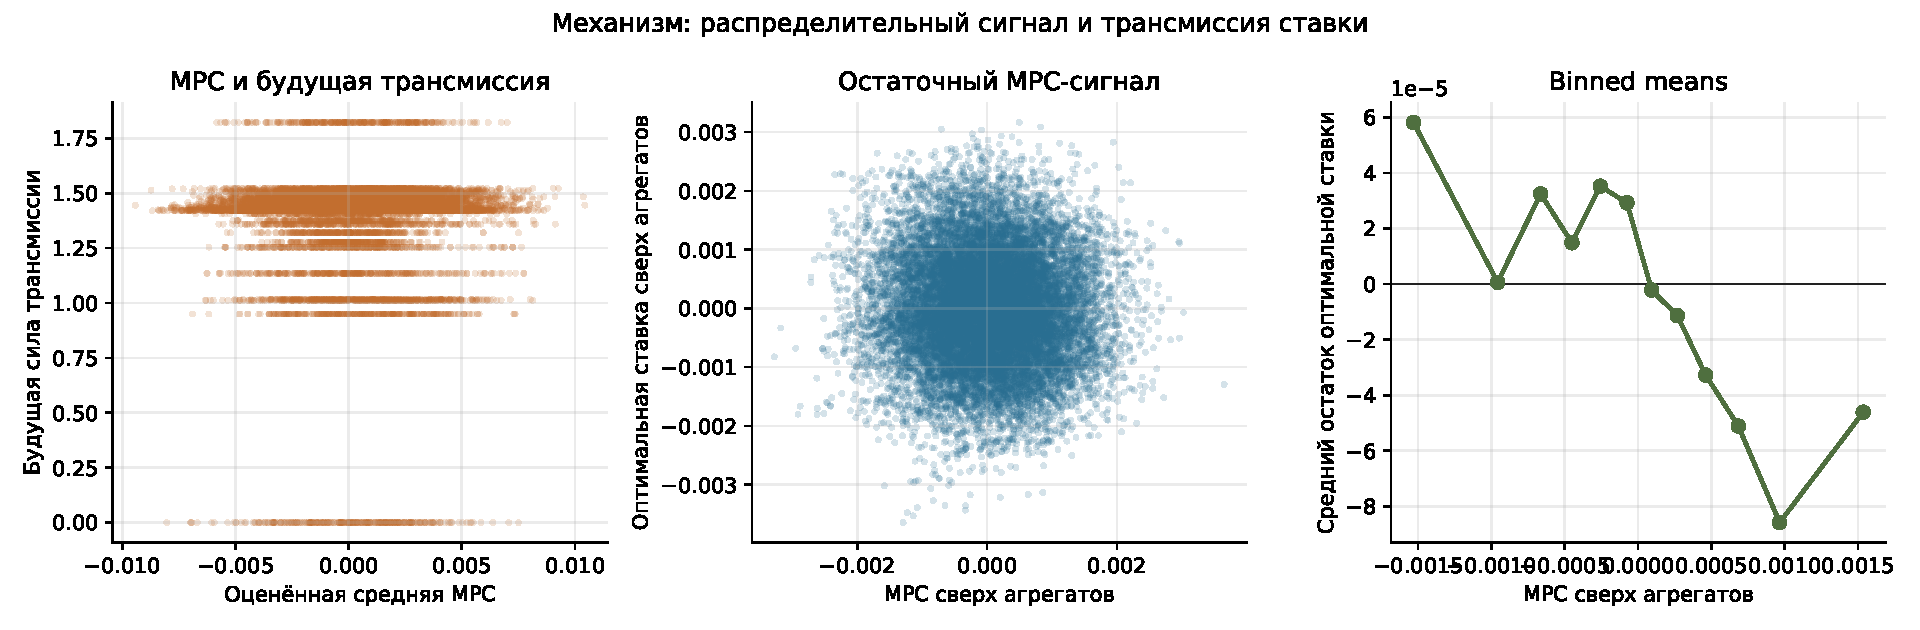
\includegraphics[width=\textwidth]{figures/fig_mechanism_distribution_transmission.pdf}
\caption{Распределительный сигнал, будущая трансмиссия и остаток оптимальной ставки}
\end{figure}

\begin{figure}[h!]
\centering
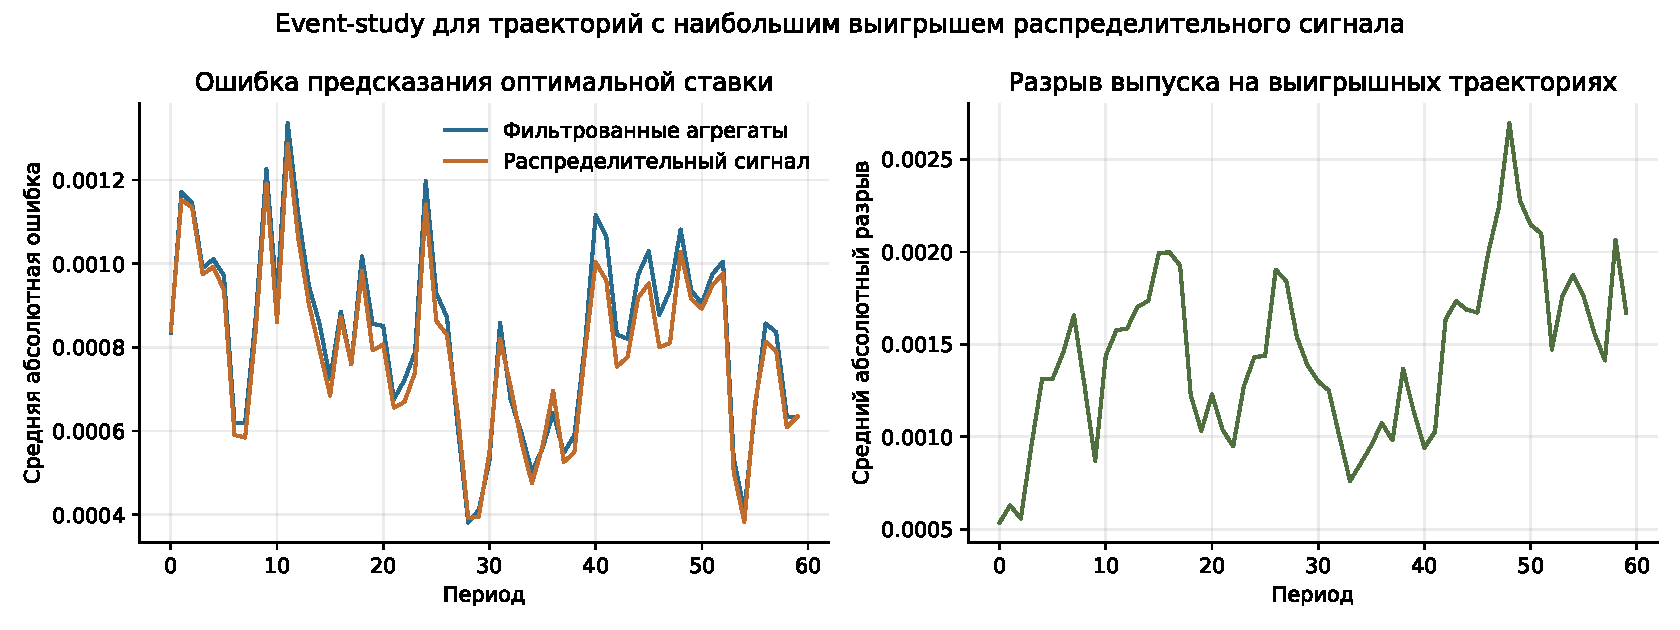
\includegraphics[width=\textwidth]{figures/fig_mechanism_event_study.pdf}
\caption{Траектории с наибольшим выигрышем распределительного сигнала}
\end{figure}

\subsection{Разложение потерь}

Разложение показывает, что основная часть выигрыша идёт через выпуск. При переходе от текущих
агрегатов к фильтрованным агрегатам общее снижение потерь равно \(0.000099\), из них
\(0.000074\) приходится на разрыв выпуска. При добавлении распределительной информации сверх
фильтрованных агрегатов общее снижение равно \(0.000055\), из них \(0.000048\) приходится на
разрыв выпуска. Компонент сглаживания ставки почти не меняется.

\subsection{Проверка с обратной связью}

В базовой локальной проекции информационные признаки берутся с исходной HANK/SSJ-траектории, а
агрегатные последствия альтернативной ставки пересчитываются через SSJ-отклики. В усиленной
проверке контрфактическое состояние, наблюдения и фильтрованные признаки пересчитываются
итеративно. Правила не переобучаются.

В режиме с обратной связью фильтрованные агрегаты дают средние потери \(0.002138\), а
фильтрованные распределительные показатели -- \(0.002098\). Знак остаётся правильным, но эффект
статистически слабее: снижение потерь равно \(0.000040\), а интервал для разности включает ноль.
Отдельные распределительные статистики выглядят устойчивее: доля низколиквидных домохозяйств и
процентная экспозиция снижают потери примерно на \(0.00031\) относительно фильтрованных агрегатов.

Эта проверка не является полной HANK-оценкой с обратной связью. В текущем наборе SSJ-якобианов
прямые отклики ставки есть для инфляции, выпуска и потребления, но не для распределительных
статистик. Поэтому для распределительных переменных используется локальная проекция на агрегатные
SSJ-эффекты. Максимальная следующая версия требует прямых SSJ-якобианов для MPC, доли
низколиквидных домохозяйств и процентной экспозиции.

\subsection{Интерпретация}

Абсолютные значения функции потерь малы, потому что эксперимент проводится вокруг стационарного
состояния и использует квадратичный стабилизационный критерий. Поэтому содержательная проверка
опирается на парные разности на одинаковых траекториях, доверительные интервалы, проверки с
ложными признаками и сравнение с полной информацией.

Итоговый вывод такой: распределительная информация имеет положительную предельную ценность в
локальной HANK/SSJ-среде, но эта ценность не должна трактоваться как автоматическое преимущество
любого расширенного набора переменных. Эффект сохраняется для остаточной распределительной
информации и исчезает или меняет знак для искусственных и временно смещённых признаков.
